\documentclass[11pt, letterpaper]{article}

% Below are some packages for the layout.
\usepackage[letterpaper, margin=1in]{geometry} % To set the layout.
\usepackage{layout} % To see the layout of the page.
%\usepackage[parfill]{parskip} % To control paragraph skips.

% Below are some packages for hyper links.
%\usepackage[bookmarksnumbered,bookmarksopen,colorlinks,citecolor=blue,linkcolor=blue,pagebackref]{hyperref}
%\usepackage[bookmarksnumbered,bookmarksopen,colorlinks,citecolor=blue,linkcolor=blue,pagebackref]{hyperref}
\usepackage[bookmarksnumbered,bookmarksopen,colorlinks,citecolor=blue,linkcolor=blue]{hyperref}
%\usepackage[bookmarksnumbered,bookmarksopen,colorlinks,citecolor=blue,linkcolor=blue,pagebackref, dvipdfm]{hyperref}

% Below are some packages for references.
\usepackage[super,comma,sort&compress]{natbib} %\usepackage{natbib}

% Below are some packages for mathematics.
\usepackage{amsfonts}
\usepackage{mathrsfs}
%\usepackage[centertags]{amsmath}
\usepackage{amsmath}
\usepackage{amssymb}
%\usepackage[framed, hyperref]{ntheorem}
\usepackage{amsthm}

% Below are some packages for colors and graphics.
\usepackage{color}
\usepackage{graphicx}

\usepackage{ifthen}
\usepackage{authblk}

\usepackage{pdflscape}



%%%%% Keywords:
\newcommand{\Keywords}[1]{\par\noindent{\small{\em Keywords\/}: #1}}


\newtheorem{example}{Example}
\newtheorem{theorem}{Theorem}

\renewcommand{\vec}[1]{\mathbf{#1}}

%\DeclareMathOperator*{\argmin}{argmin}
\newcommand{\argmin}{\text{argmin}}
\newcommand{\diag}{\text{diag}}
\newcommand{\E}{\mathbb{E}}
\newcommand{\bd}[1]{\boldsymbol{#1}}
\newcommand{\Pn}{\mathbb{P}_{n}}







\begin{document}

\title{Simple and intuitive optimal risk thresholds for a single screen: \\The next step after a Decision Curve Analysis}

%\author[1]{Authors}
\author[1]{Hormuzd A. Katki}
\affil[1]{Division of Cancer Epidemiology and Genetics, National Cancer Institute, Rockville, MD}
\author[2]{Ionut Bebu}
\affil[2]{Biostatistics Center, George Washington University, Rockville, MD, USA}%\date{}
\maketitle



%%% ----------------------------------------------------------------------
\setcounter{page}{1}   % begin to count from 1.
\pagenumbering{roman}   % assign the numbering system.

\setcounter{tocdepth}{3} % Set the depth of the contents.


%\tableofcontents
%\listoffigures % Have the list of figures.
%\listoftables % Have the list of tables.



\begin{abstract}
\noindent \textbf{Introduction:}  Decision Curve Analysis (DCA) is a modern popular approach to identify the range of risk thresholds at which screening with a biomarker is the best decision.  However DCA does not directly account for costs and effectiveness of subsequent interventions, and most applications assume a costless screening biomarker for simplicity.  We develop a simple framework that accounts for costs and effectiveness to identify optimal cost-effective thresholds for a single screen, and compare to findings from DCA.

\noindent\textbf{Methods:}  We calculate the Incremental Net Benefit (INB) for a single-time screen as a function of costs (screening test, definitive confirmatory test, and subsequent interventions) and effectiveness (dollar value of life-years gained by undergoing interventions).  We provide a simple expression for the optimal cost-effective risk-threshold and for the dollars per life-year gained threshold associated with an optimal risk-threshold.  We apply our framework to the controversy over using the BRCAPRO risk model to screen women for mutations in \textit{BRCA1/2} that cause high risks of breast and ovarian cancers. Mutations are rare in the general population, but more common among Ashkenazi-Jews. 

\noindent\textbf{Results:}  According to DCA, assuming costless BRCAPRO, optimal risk thresholds from 1\%-30\% support using BRCAPRO to screen among Ashkenazi-Jews.  However, our framework shows that these optimal risk-thresholds are  infeasible because they imply a negative dollars per life-year gained threshold.  Furthermore, DCA is sensitive to a small cost of shared decision-making with BRCAPRO (\$100), which is hard to detect by DCA but easily seen by INB.    In the general population, optimal risk thresholds from 0.12\% to 0.91\% support screening.  However, these optimal thresholds represent dollars per life-year gained thresholds of \$16,000 to \$306,000, suggesting that none or only some of the optimal thresholds are feasible in practice, where threshods below \$100,000 are typical.

\noindent\textbf{Limitations:}  Our framework requires specifying costs of tests and interventions, and the value of life-year gained.

\noindent\textbf{Conclusions:}  Our simple framework identifies sensitivity of DCA to biomarker test costs that is hard to see by DCA.  Optimal risk thresholds identified by DCA may be infeasible based on their associated dollars per life-year gained threshold.  Our simple approach is the next step after DCA to better identify optimal cost-effective risk-thresholds.

\end{abstract}

\Keywords{
	AUC; \textit{BRCA1}; \textit{BRCA2}; cost effectiveness; decision analysis; Decision Curves; Diagnostic Testing; Incremental Net Benefit; Net Benefit; risk prediction ; ROC; Screening; Youden's index.
}




\setcounter{page}{1}    % setting the count number.
\pagenumbering{arabic}  % assigning another numbering system.



%%%%%%%%%%%%%%%%%%%%%%%%%%%%%%%%%%%%%%%%%%%%%%%%%%%%%%%%%%%%%%%%%%%%%%%%%%
%%%%%%%%%%%%%%%%%%%%%%%%%%%%%%%%%%%%%%%%%%%%%%%%%%%%%%%%%%%%%%%%%%%%%%%%%%

% https://mdm.uic.edu/manuscript-requirements/

\section{Introduction}
\label{sec:intro}
In population disease screening, a cheap, non-invasive, but imperfect test is conducted on a population to determine who should be referred for tests that are definitive for the presence of disease.   Because screening tests are imperfect indicators of the presence of disease, the goal is choose a screening test threshold that is cost-effective at controlling the rates of false classification.  

There is much literature on identifying cost-effective thresholds, such as the classic paper of Pauker and Kassirer~\citep{Pauker1980}.  The cost-effective threshold depends on the costs, benefits, and harms of the tests and subsequent interventions.  Subsequent mathematical developments conglomerate costs, benefits and harms into “utilities” that are even harder to specify~\citep{Gail2005,Baker2009a}.  However, statistical metrics that do not require costs, benefits, and harms, such as Youden’s index, AUC, and Mean Risk Stratification, cannot identify cost-effective thresholds.  The important recent advance of Net Benefit~\citep{Vickers2006} in practice typically assumes costless screening tests, and considers risk-thresholds as a sensitivity analysis and thus also cannot identify cost-effective thresholds.

In contrast, a full decision analysis, specifying costs, benefits, and the monetary value of life, can determine cost-effective thresholds.  However, usually these analyses require complex decision trees and microsimulation to evaluate the situation as comprehensively as possible.  In such analyses, it can be hard to glean intuition about which quantities are most important, even when probabilistic sensitivity analysis is conducted.  To complement such comprehensive decision analyses, there is a need for an approach to risk thresholds that is simple, transparent, provides a reasonable estimate of the range of realistic cost-effective thresholds, and provides simple intuition on which quantities are most important.  

We propose a simple framework that identifies the cost-effective risk threshold for a single-time screen, such as screening for gestational diabetes, syphilis in pregnancy, or genetic mutations.  We show that the Incremental Net Benefit (INB) depends on only 3 quantities: the costs of the screening test and definitive test, and a parameter we call the net effectiveness of early intervention (NE).  We show that the cost-effective risk-threshold for the screening test depends on only the cost of the definitive test and the NE.  Our framework also provides a simple criterion, based on the slope of the Lorenz curve, for judging when one screening test is more cost-effective than another.

We apply our framework to the controversy over the risk-threshold to identify who should get testing for mutations in the \textit{BRCA1/2} genes, which cause high risks of breast and ovarian cancer~\citep{Kuchenbaecker2017}.   Current US and UK guidelines refer women for mutation testing only if they have a strong family history of breast or ovarian cancer~\citep{Moyer2014}, as quantified by a risk model calculating that their risk of carrying a \textit{BRCA1/2} mutation exceeds 10\%~\citep{NICE2017}.  However, as mutation-testing costs plummet, prominent voices have called for testing \textit{all} women~\citep{King2014}, equivalent to a 0\% risk-threshold.   The Screen Project offers \textit{BRCA1/2} testing to any Canadian~\citep{TheScreenProject2017}.  In a landmark ruling, the US FDA recently authorized direct-to-consumer genetic testing, for \textit{BRCA1/2} mutations among Ashkenazi-Jews~\citep{Rabin2018}.  Population mutation screening is inevitable, but there are strong disagreements on how such programs should be conducted.

We recently showed that 80\% of Ashkenazi-Jewish mutation-carriers could be identified by testing only 44\% of Ashkenazi-Jewish women~\citep{Best2019} at highest risk for carrying mutations, as identified by the BRCAPRO~\citep{Parmigiani1998} risk model.  This is achieved by a low mutation-risk threshold of 0.78\%, far lower than the current 10\% US and UK guideline.  We previously examined multiple statistical metrics, such as AUC, Net Benefit, and Mean Risk Stratification, to examine properties of different risk thresholds.  However, no statistical metric can formally identify optimal cost-effective risk-thresholds.  In this paper, we input costs and benefits into our simple framework to identify optimal risk thresholds to screen women for referral for \textit{BRCA1/2} genetic testing.  Using our simple framework, our findings are comparable to more comprehensive, but more complex and less transparent, microsimulation approaches to this issue~\cite{Long2015,Manchanda2015}.   In this example, we show that Net Benefit is sensitive the standard assumption of a costless screening test and the ranges of risk thresholds identified as being favorable for screening can imply unrealistic values for dollars per life-year gained.

%For Ashkenazi-Jews, the range of risk thresholds identified by Net Benefit as favoring screening is misleading because the dollars per life-year gained implied by these thresholds is negative and thus not allowable.  This means that performing BRCA1/2 genetic testing on all Ashkenazi-Jewish women would save money versus using BRCAPRO to screen to identify who should get genetic testing.


%This is the basis for recent developments in risk prediction metrics, such as Net Benefit.  In current approaches, the utilities are left unspecified and all possible risk thresholds are considered as a sensitivity analysis.  Because costs, benefits and harms require specification, we propose that scientists who evaluate new medical tests or propose thresholds for test must try to specify these as best as possible.  

\section{A cost-effectiveness framework for a single-time screen}

\subsection{Defining average costs and effectiveness for a single-time screen} 
\label{sec:framework}

In screening, asymptomatic people are given the single screening test.  Two outcomes are possible:
\begin{enumerate}
	\item If the test is positive, the person is referred for definitive disease testing.  If disease is diagnosed, it is then treated.  Because the screening test found the disease early (i.e. in the absence of symptoms), presumably treatment is more effective than for disease found later on the basis of symptoms.
	
	\item If the test is negative, there is no further action.  However, future symptoms will prompt definitive testing to diagnose disease.  If disease were diagnosed in the future, presumably treatment is less effective than it would have been had disease been found earlier.
\end{enumerate}

\noindent Four parameters define the average costs for a single screen:
\begin{enumerate}
	\item Let $c_m$ denote the cost of screening marker evaluation.
  The screening test is imperfect, else it would be the definitive test.  The main goal of our paper is to identify the cost-effective threshold for deciding screening test positivity.
	
	\item Let $c_0$ denote the cost of the definitive test for disease, e.g. biopsy or imaging.  We presume this test is perfect but is so invasive and costly that practically it cannot be the screening test.

	\item Let $c_1$ be the cost of treatment for a disease case diagnosed early.  This occurs for those testing positive for disease on both the screening test and definitive test.

	\item Let $c_2$ be the treatment cost for a cancer case diagnosed late.  This occurs for those with negative screening test (or not screened at all), but in the future develop symptoms and disease is diagnosed by the definitive test.
\end{enumerate}

\noindent Three parameters  define the average effectiveness of a single screen, defining effectiveness as the value of the gain in life-expectancy:
\begin{enumerate}
	\item Let $e_0$ be the life-expectancy for someone who never develops disease 
	
	\item Let $e_1$ be the life-expectancy for someone with a positive marker $M$ who then tests positive for disease.  This is early-detection and is the benefit of screening.
	
	\item Let $e_2$ be the life-expectancy for someone who is either not screened or tests screen-negative, but then develops disease.  This is late detection and is a screening failure.  We presume that $e_1 \ge e_2$, else screening causes obvious harm. 
\end{enumerate}
Finally, the effectiveness “value” must be on the same scale as costs, and we call $d$ the dollar-value of 1 life-year.  In our examples of population mutation-screening and CT lung-cancer screening, we derive the 4 cost and effectiveness parameters $e_1$ and $e_2$ (we show that $e_0$ does not require specification).  We propose sensitivity analyses for costs and effectiveness and, in the Discussion, we consider practical weaknesses of our approach to identifying costs and effectiveness.

\subsection{Calculating Incremental Net Benefit (INB)}
\label{sec:INB}

The INB is the difference in average costs and effectiveness of a 1-time screen versus never screening.  Define disease as $D$ and the marker for the screening test as $M$. 
\begin{enumerate}
	\item{No screening for $M$.  There are two possibilities:
		\begin{enumerate}
			\item{The individual has disease ($D+$): cost is $c_0+c_2$ and effectiveness is $d\cdot e_2$}
			\item{The individual does not have disease ($D-$): cost is 0, effectiveness is $d\cdot e_0$.}
		\end{enumerate}
	}
	\item{Screening for $M$.  The marker is dichotomized as positive ($M+$) and negative ($M-$) based on a underlying threshold $m_0$ (our goal is to identify the cost-effective $m_0$).  There are four possibilities:
		\begin{enumerate}
			\item{True Positive: The screening is positive and the individual has disease ($M+,D+$). \\ Cost is $c_m+c_0+c_1$ and effectiveness is $d\cdot e_1$.}
			\item{False Positive: The screening is positive but the individual does not have disease ($M+,D-$).  Cost is $c_m+c_0$ and effectiveness is $d\cdot e_0$.}
			\item{False Negative: The screening is negative but the individual has disease ($M-,D+$).  \\Cost is $c_m+c_0+c_2$ and effectiveness is $d\cdot e_2$.}
			\item{True Negative: The screening is negative and the individual has not have disease ($M-,D-$).  Cost is $c_m$ and effectiveness is $d\cdot e_0$.}
		\end{enumerate}  
	}
\end{enumerate}

\noindent Let $C$ and $E$ be the average cost and effectiveness w/o screening, and $C_M$ and $E_M$ with screening:
\begin{eqnarray*}
	{\cal E} (C) &=& (c_0+c_2)\cdot P(D+) \\
	{\cal E} (E) &=& d[e_2\cdot P(D+) + e_0\cdot P(D-)] \\
	{\cal E} (C_M) &=& c_m + [1-P(D-,M-)]\cdot c_0+P(D+,M-)\cdot c_2+P(D+,M+)\cdot c_1\\
	{\cal E} (E_M) &=& d[e_0\cdot P(D-) + P(D+,M+)\cdot e_1 + P(D+,M-)\cdot e_2].
\end{eqnarray*}
The differences in cost and effectiveness between screening and never screening are:
\begin{eqnarray*}
	\Delta C &=& c_m + c_0\cdot P(M+) + (c_1 - c_2 - c_0)\cdot P(D+,M+)\\
	\Delta E &=& d(e_1 - e_2)\cdot P(D+,M+).
\end{eqnarray*}

\noindent The Incremental Net Benefit is
\begin{eqnarray} 
INB &=& \Delta E - \Delta C\\ \nonumber
&=& [d(e_1-e_2)-(c_1-c_2-c_0)]P(D+,M+) - c_m - c_0P(M+)\\ \nonumber
&=& [e+c_0]P(D+,M+) - c_m - c_0P(M+), \label{eq:INB}
\end{eqnarray}
where $e = d(e_1-e_2)-(c_1-c_2)$ is the "net effectiveness of early intervention". The net effectiveness contrasts the dollar-value of the life-expectancy gain with dollar increase in treatment cost for early vs. late detection.  If net effectiveness $e<0$, screening is never cost-effective (See Appendix).  

The INB reveals that only certain aspects of costs and effectiveness require specification. First, only the dollar-value of life-years gained $d(e_1-e_2)$ requires specification.  Life-expectancy in the absence of disease ($e_0$) is not needed.  Second, only the difference of early vs. late treatment costs $c_1-c_2$ requires specification.  Importantly, if treatment costs were similar regardless of early versus late detection, or if treatment costs are far below the dollar value of life-years gained, then net effectiveness approximately depends only only the value of life-years gained.


\subsection{Optimal cost-effective risk threshold that maximizes INB}
\label{sec:optimalthreshold}

The optimal risk threshold can be derived from the classical expected utility approach~\citep{Pauker1980}.  Calculating expected utility requires specifying the utility for the 4 possible outcomes: the utility of true positive prediction $U_{TP}$, the utility of true negative prediction $U_{TN}$, the utility of false positive prediction $U_{FP}$, and the utility of false negative prediction $U_{FN}$.  These utilities are the difference of effectiveness and cost for each of the 4 outcomes in Section~\ref{sec:framework}:
\begin{eqnarray*}
	U_{TP} &=& d\cdot e_1 - (c_m+c_0+c_1) \\
	U_{FN} &=& d\cdot e_2 - (c_m+c_0+c_2)\\	
	U_{TN} &=& d\cdot e_0 - (c_m)\\
	U_{FP} &=& d\cdot e_0 - (c_m+c_0)
\end{eqnarray*}
The marker/model is dichotomized at cutpoint $m_0$ that defines a risk threshold $R$: $P(D+|M=m_0)=R$.  The $R$ that maximizes expected utility is determined by benefit ($B=U_{TP}-U_{FN}$) and cost ($C=U_{TN}-U_{FP}$), and is known to be $R=C/(B+C)$~\citep{Pauker1980}.  For a single screen, note that $B=e$ and $C=c_0$.  Thus the optimal cost-effective risk-threshold is
\begin{eqnarray}
R &=& \frac{C}{B+C} = \frac{c_0}{e+c_0}.
\end{eqnarray} 
The WebAppendix derives this optimal threshold from first principles.

The value of this expression is that it does not require 4 abstract uncalculable utilities, but only 2 concrete calculable quantities: the definitive test cost $c_0$ and the net effectiveness of early intervention $e=d(e_1-e_2)-(c_1-c_2)$.  In the following examples, we obtain $c_0$ and $e$ from data to directly propose optimal thresholds for lung-cancer screening and population mutation-screening.

Also, neither screening test characteristics nor disease prevalence matter for calculating the optimal risk-threshold.  This is unlike metrics such as MRS, Youden's index, AUC, Vickers's Net Benefit gain, which are all maximized at risk threshold equals disease prevalence (i.e $R=P(D+)$), regardless of costs and effectiveness. 

Also, the optimal risk threshold $R$ does not require the screening test cost $c_m$, because risk thresholds only matter after the screening test is conducted, and thus the screening test cost is a sunk cost.  However, the screening test cost matters to check if screening is better than screening no one or testing everyone (see Section~\ref{sec:INBgain}).  




\subsection{Gain in INB  versus screening no one or testing everyone}
\label{sec:INBgain}

If $INB(R)>0$, then screening based on the marker is more cost-effective than screening no one.  To also check if screening is also more cost-effective than just conducting the definitive test on everyone, we have to compare the INB versus the INB for testing everyone versus screening no one, called $INB_{all}$.   For testing everyone, we have $P(D+,M+)=P(D+)$, $P(M+)=1$, and $c_m=0$ since we don't need the screening test.  Plugging these into equation~\ref{eq:INB} yields $INB_{all}=(e+c_0)P(D+)-c_0$.  The $INB_{Gain}$ is the increase in INB beyond either screening no one or testing everyone:
\begin{eqnarray}
INB_{Gain}(R) = INB(R) - max(0,INB_{all}).
\end{eqnarray}
Risk thesholds where $INB_{Gain}(R)>0$ are thresholds where screening is better than screening no one or testing everyone.

\subsubsection{Comparison of INB to Net Benefit (NB)}
\label{sec:NB}

Net Benefit (NB) is a well-known and important approach to identify risk thresholds where using a test to decide who should get treated is better than treating no one or everyone~\citep{Vickers2006}.  NB equals the INB standardized by benefit $B=e$ (see Appendix).  We define $NB_{Gain}$ as the $INB_{Gain}$ standardized by benefit $B=e$, as a function of optimal risk threshold $R$:
\begin{eqnarray*}
	N\!B_{Gain}(R) = N\!B(R) - max(0,INB_{all}/e) = N\!B(R) - max(0,P(D+)/(1-R)-R).
\end{eqnarray*}
The thresholds $R$ where $N\!B_{Gain}(R)>0$ are thresholds where the risk model is better than screening no one or testing everyone.  These are the same thresholds as where $INB_{Gain}(R)>0$.  The advantage of NB over INB is that, for a costless test $c_m=0$, one does not need to specify net effectiveness of early intervention $e$ (see Appendix), so that only risk threshold $R$ is required.  All applications of NB we are aware of assume a costless test.   However, every test in reality has some cost.  We will compare INB to NB to show the value of explicitly specifying costs and effectiveness.  


%\subsection{INB versus testing everyone}
%\label{sec:INBvsAll}
%
%We must also compare screening versus conducting the definitive test on everyone in the population.  As noted in the introduction, this is relevant to genetic testing, where the costs of genetic testing is becoming so cheap that there are calls to simply test everyone.  Everyone undergoes definitive testing, but all prevalent disease is detected early:
%\begin{enumerate}
%	\item{The individual has disease ($D+$): cost is $c_0+c_1$ and effectiveness is $e_1$}
%	\item{The individual does not have disease ($D-$): cost is $c_1$, effectiveness is $e_0$.}
%\end{enumerate}
%Following the argument of section~\ref{sec:INB}, the INB comparing screening versus testing everyone is
%\begin{eqnarray}
%INB_{all} &=& -[e+c_0]P(D+,M-) - c_m + c_0P(M-).
%\end{eqnarray}
%For screening to be the best decision, both $INB>0$ and $INB_{all}>0$.


\section{Example: Who should undergo \textit{BRCA1/2} genetic testing?}
\label{sec:BRCA}

\subsection{Background}
\label{sec:BRCAbackground}

As detailed in the Introduction, mutations in the \textit{BRCA1/2} genes cause high risk of breast and ovarian cancers.  The mutations are rare in the general population ($\approx0.26\%$), but much more common among Ashkenazi-Jews ($\approx2.3\%$).  Currently, women are asked to provide their family history of cancer (e.g. see Webappendix), and she is offered mutation-testing in the UK and US if a risk model calculates that her risk of carrying a mutation exceeds 10%~\citep{NICE2017}.  We focus on the BRCAPRO~\citep{Parmigiani1998} risk model.  

However, as mutation-testing costs plummet, prominent voices have called for testing all women, which would strain clinical resources by testing millions of women, 99.75\% of whom will test negative.  Instead, a lower risk threshold, below 10\%, might identify most all mutation-carriers, yet avoid unnecessary testing for most women.  We recently showed that a low 0.78\% risk-threshold would identify 80\% of Ashkenazi-Jewish mutation-carriers yet test only 44\% of Ashkenazi-Jewish women~\citep{Best2019}.  However, we could not formally justify any choice of risk-threshold.  Here we examine cost-effectiveness of possible risk thresholds.

%There is great controversy over who should get tested for mutations in the \textit{BRCA1/2} genes, which cause high risks of breast and ovarian cancer.  The mutations are rare in the general population ($\approx0.25\%$), but are 10 times more common among Ashkenazi-Jews~\citep{STRUEWING1997}.  Currently, women are referred for mutation testing only if they have a strong family history of breast or ovarian cancer~\citep{Moyer2014}, as quantified by a risk model calculating that their risk of carrying a mutation exceeds 10\%~\citep{NICE2017}.  However, as mutation-testing costs fall, prominent voices have called for testing \textit{all} women~\citep{King2014,GenomeWeb2017a}. Testing all women would strain clinical resources by testing millions of women, $99.75\%$ of whom will test negative.  At US \$500-\$1,000 per test, testing millions of women has clear commercial implications.  
%
%In contrast, we recently demonstrated that 80\% of Ashkenazi-Jewish mutation-carriers could be identified by testing only 44\% of Ashkenazi-Jewish women~\citep{Best2019}.  This is achieved by a low mutation-risk threshold of 0.78\%, far lower than the current 10\% recommendation.   However, we could not formally justify any choice of risk-threshold.  Here we examine cost-effectiveness of possible risk thresholds.

We used data on 4,589 volunteers (102 \textit{BRCA1/2} mutation carriers) from the Washington Ashkenazi Study (WAS)~\citep{STRUEWING1997}.  We calculated each volunteer's risk of carrying a mutation, based on their self-reported family-history of breast/ovarian cancers, using the BRCAPRO risk model~\citep{Parmigiani1998}.  Here $M$ is the BRCAPRO risk score, and because BRCAPRO is a well-calibrated risk model~\citep{Best2019}, $m_0=R$, i.e. the cutpoint $m_0$ equals the risk threshold $R$. Disease $D$ indicates the presence of a \textit{BRCA1/2} mutation.  We use previously published methodology to use WAS data to also calculate BRCAPRO risk scores valid for the general population~\citep{Best2019} (see WebAppendix).

%\textit{BRCA1/2} mutation-carriers have 5.7 fewer years of expected life~\citep{Mai2009}.  

\subsection{Costs and effectiveness for \textit{BRCA1/2} mutation screening}
\label{sec:CostsEffBRCA}

We set life-years gained $e_1-e_2$ as 5.0 life-years, which is the estimate for removing both ovaries and breasts (followed by frequent cancer screening) in a 50-year old mutation-carrier who has completed childbearing.  We use costs used by the Long and Ganz decision analysis from 2015~\citep{Long2015} to compare results (In section ?? we update to current costs).  We set $c_m$ as the cost of using the BRCAPRO risk model, which is "free" but requires a doctor's visit to assess family history, costing roughly $c_m=\$100$.  For the cost of BRCA genetic testing $c_0$,  for Ashkenazi-Jews, the cost is now $c_0=\$249$, but non-Ashkenazim require full gene sequencing which costs $c_0=\$2200$.   For treatment costs, $c_1$ is the cost of removing the breasts and ovaries and the average treatment cost for the rare breast or ovarian cancers that occur anyway.  For $c_2$, this is the cost of cancer treatment for mutation carriers who are not found until cancer is diagnosed.  By~\citep{Long2015}, $c_1=\$28393$ and average cancer treatment cost is $c_2=\$187110$ (see WebAppendix).

\subsection{\textit{BRCA1/2} mutation screening for Ashkenazi Jews}
\label{sec:BRCAAJs}

\subsubsection{INB gain versus NB gain}
\label{sec:INBvsNB}

\begin{figure}[t!]
	\centering
	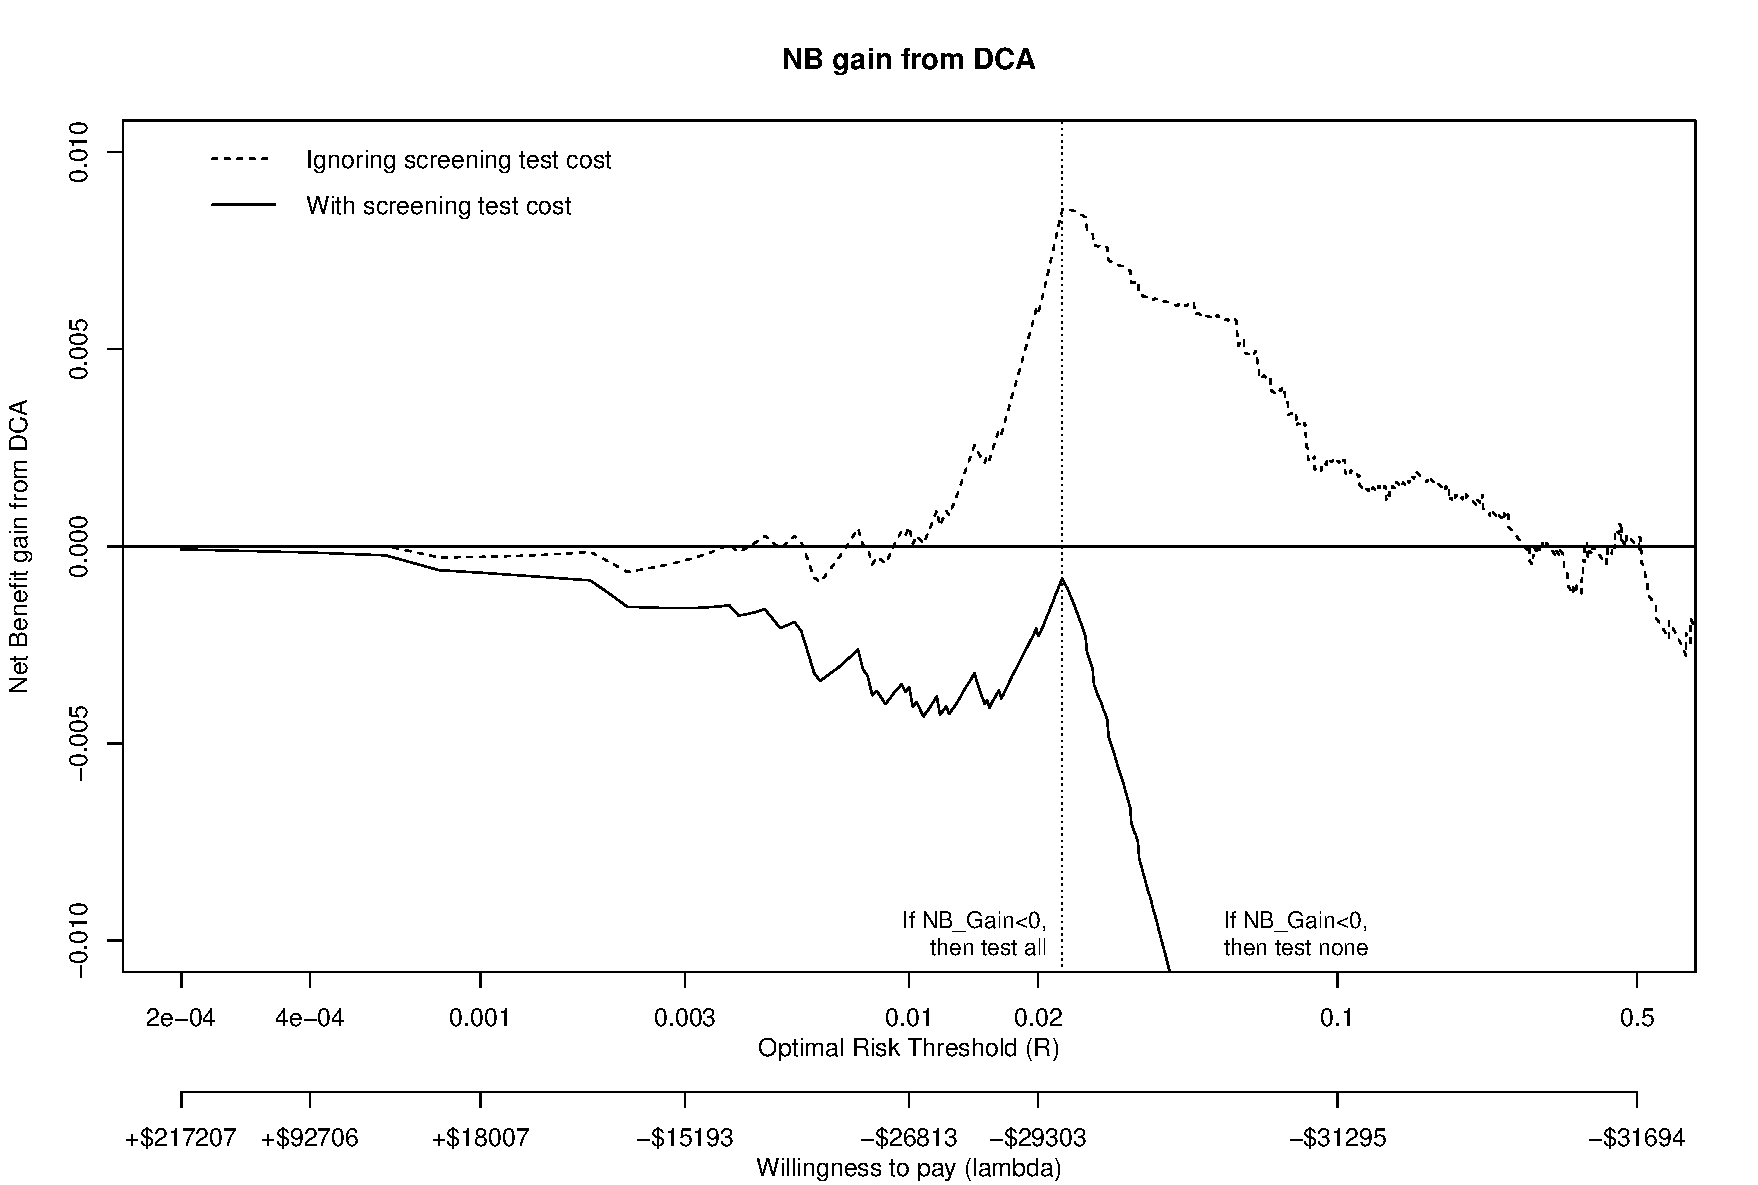
\includegraphics[angle=-0,width=6.5in,]{testcostsAJ.pdf}
	\caption{INB gain (left panel) and NB gain (middle panel) vs. BRCAPRO risk-threshold for using the BRCAPRO risk model to screen for which Ashkenazi-Jews should get \textit{BRCA1/2} genetic testing.  The right panel plots NB gain for a costless BRCAPRO screening test versus the dollars per life-year gained implied by each optimal risk-threshold.}
	\label{fig:testcostsAJ}
\end{figure}

Figure~\ref{fig:testcostsAJ} shows that the INB gain (left panel) and NB gain with BRCAPRO screening test cost $c_m=\$100$ (middle panel) are always negative.  Thus screening is never the best choice.  However, the NB gain estimated by usual costless test assumption (middle panel) shows that screening is the best choice for a wide range of risk thresholds from 1\% to 30\%.  Thus \textit{BRCA1/2} mutation screening is sensitive to a small BRCAPRO screening test cost.  It is hard to see this sensitivity from the costless NB gain because its units are abstract.  In contrast, this sensitivity is easy to see from INB gain because its units are dollars.  The INB asymptotes at -\$100, clarifying that a screening test that was just \$100 cheaper would permit screening at a wide range of risk-thresholds.

\subsubsection{Dollars per life-year gained implied by optimal risk-thresholds}
\label{sec:DollarsPerLYG}

Fixing costs and life-years gained, an optimal risk threshold implies a threshold for dollars per life-year gained.  Because
\begin{eqnarray*}
	R = \frac{c_0}{e+c_0} = \frac{c_0}{d(e_1-e_2)-(c_1-c_2) +c_0},
\end{eqnarray*}
where $d$ is the dollars per gain in life-years $(e_1-e_2)$, then
\begin{eqnarray}
\label{eq:dollarsperLYG}
	d = \frac{c_0(1-R)/R + (c_1-c_2)}{e_1-e_2}.
\end{eqnarray}
Figure~\ref{fig:testcostsAJ} (right panel) plots NB (for a costless BRCAPRO test) versus the threshold for dollars per life-year gained.   Surprisingly, the wide range of risk thresholds supporting screening for a costless BRCAPRO test implies that the threshold for dollars per life-year gained is \textit{negative}.  This means that screening with BRCAPRO at optimal thresholds actually costs more than doing genetic testing on all Ashkenazi-Jewish women, which agrees with other decision analyses~\citep{Long2015,Manchanda2015}.   This striking example demonstrates that optimal risk thresholds can imply unrealistic thresholds of dollars per life-year gained and demonstrates a weakness in any approach that examines only risk thresholds and not dollars per life-year gained thresholds.  Note that dollars per life-year gained thresholds cannot be calculated by Net Benefit and requires specifying costs and effectiveness.

The reason for the negative dollars per life-year gained is that $c_1-c_2=-\$158717$ is strongly negative.  This is not overcome by the cost increase due to genetic testing because $c_0$ is only $\$249$, the smallest optimal threshold is $R\approx1\%$, and thus $c_0(1-R)/R\approx\$25000$ . Thus we immediately see that the reason why testing all Ashkenazi Jews saves money versus screening with BRCAPRO is because treating cancer is far more expensive than all costs incurred by genetic testing.  

Our simple framework easily allows for other calculations of interest.  For example, the maximum cost of genetic testing to ensure that testing everyone saves money versus screening at an optimal risk threshold of 1\% is approximately $(c_1-c_2)R/(1-R)=\$158717/99\approx\$1600$.  


\subsection{\textit{BRCA1/2} mutation screening for the general population}
\label{sec:BRCAgenpop}

\begin{figure}[t!]
	\centering
	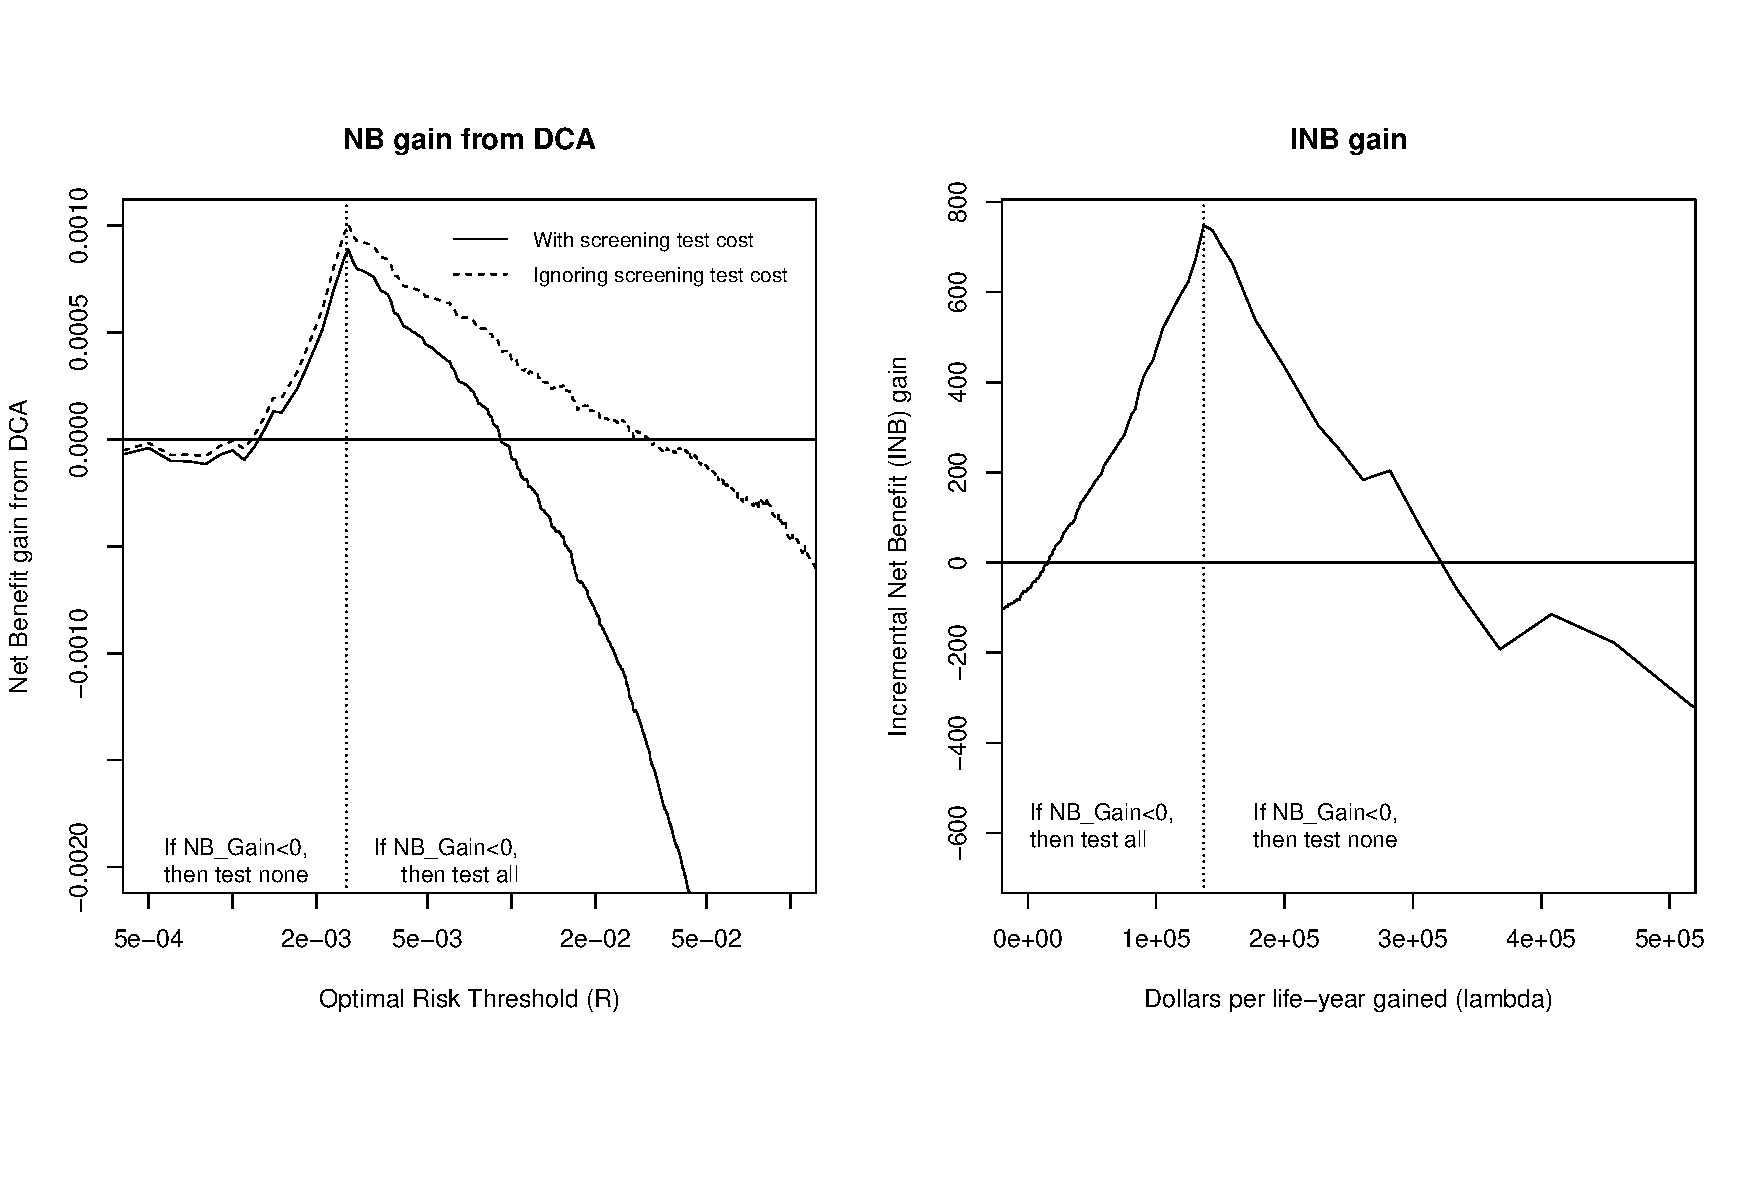
\includegraphics[angle=-0,width=6.5in,]{testcostsGenPop.pdf}
	\caption{NB gain vs. risk-threshold (left panel) and INB gain vs. dollars per life-year gained (right panel) for using the BRCAPRO risk model to screen for which members of the general population should get \textit{BRCA1/2} genetic testing.}
	\label{fig:testcostsGenPop}
\end{figure}

In the general population, \textit{BRCA1/2} mutations have only 0.26\% prevalence (10 times fewer than in Ashkenazi-Jews).  Figure~\ref{fig:testcostsGenPop} (left panel) shows that accounting for just a \$100 screening BRCAPRO test cost greatly reduces the range of allowable risk thresholds for screening, from $(0.12\%,3.1\%)$ to $(0.13\%,0.91\%)$.  Figure~\ref{fig:testcostsGenPop} (right panel) shows that screening with BRCAPRO is cost-effective at dollars per life-years gained thresholds ranging from $(\$16,\!000,\$306,\!000)$, which spans typical thresholds for Western countries.  The peak INB of \$700 shows that a BRCAPRO screening that cost \$700 more (total $c_m=\$800$) would be required to wipe out any possibility of screening, which is unreasonably expensive for shared decision-making.  

The more comprehensive analysis of Long and Ganz~\cite{Long2015} suggests that testing everyone is cost-effective at \$920,000 per QALY.  Most of this increase is due to quality adjustment, which roughly halved the value of life-years gained.  If we halve the life-years gained due to screening (to 2.5), then testing everyone is cost-effective at \$612,000 per life-year gained, much closer to Long and Ganz~\cite{Long2015}.  The complementary value of our approach is that it is 

The dollars per life-year gained at peak INB is $\$137,\!000$, which is high even for the US.  Figure~\ref{tab:dollarsperLYG} shows the performance of screening along the range of allowable thresholds of dollars per life-year gained.  As dollars per life-year gained increases, so does the fraction of mutation carriers identified (sensitivity; from 40\% to 67\%) but also the fraction of women referred for genetic testing (6.4\% to 28\%).  Note that sensitivities below 40\% do not support screening (instead screen none: sensitivity is 0\%) and neither do sensitivities above 67\% (instead test everyone; sensitivity is 100\%) The predictiveness of BRCAPRO increases from AUC of 0.669 to 0.698 at peak INB, then levels off.  

A simple calculation also shows that the maximum cost of genetic testing for testing everyone to save money versus screening at an optimal risk threshold of 0.26\% is approximately $\$158717/384\approx \$413$.  Although genetic sequencing costs are rapidly decreasing, it may be some time before \$400 can be profitably achieved.  Our simple framework easily enables such calculations. 

\begin{figure}[t!]
	\centering
	\begin{verbatim}
 Dollars/LYG Threshold INBgain Positivity      PPV     cNPV   Sens   Spec    AUC
       20197    0.0084   27.74    0.06377 0.016048 0.001640 0.4000 0.9371 0.6685
       50835    0.0053  171.90    0.09364 0.012295 0.001553 0.4500 0.9073 0.6786
      101150    0.0033  482.62    0.12929 0.010059 0.001445 0.5083 0.8717 0.6900
      137047    0.0026  748.35    0.14741 0.009401 0.001375 0.5417 0.8536 0.6976
      199395    0.0019  436.65    0.18377 0.008006 0.001332 0.5750 0.8172 0.6961
      306278    0.0013   76.46    0.28016 0.006164 0.001155 0.6750 0.7209 0.6979
	\end{verbatim}
	\caption{Peformance of using BRCAPRO to screen for \textit{BRCA1/2} mutations at various dollars per life-year gained thresholds that favor screening in the general population.}
\label{tab:dollarsperLYG}
\end{figure}


\section{Simple condition for a screening test to have greater INB}
\label{sec:moreINB}

%If one screening test has greater sensitivity and greater specificity than another, then it is obvious that first test is better without any cost-effectivenss analysis.  However, 

IONUT:  I DON'T THINK THIS FITS IN HERE.  I THINK IT SHOULD BE ITS OWN PAPER.

Usually one screening test has better sensitivity but another has better specificity.  Informational metrics like Youden's index, MRS, AUC, and NB do not explicitly consider costs and effectiveness and are all optimized when risk threshold equals disease prevalence.  Ideally, the sensitivity vs. specificity tradeoff would be evaluated considering costs and effectiveness via the INB.

For two markers $M_1$ and $M_2$ with equal marker cost, then $\Delta INB=INB_1-INB_2>0$ if
\begin{eqnarray*}
	\Delta INB &=& (e+c_0)[P(D+,M_1+)-P(D+,M_2+)] - c_0[P(M_1+)-P(M_2+)]\\
	&=& (e+c_0)[Sens_1-Sens_2]\pi - c_0[p_1-p_2] > 0
\end{eqnarray*}
for disease prevalence $P(D+)=\pi$, sensitivities $Sens_i=P(M_i\!+|D+)$, and test-positivities $P(M_i+)=p_i$.  Choosing test 1 so that $Sens_1>Sens_2$, then presuming $p_1>p_2$,
\begin{eqnarray}
\label{eq:SensMoreINB}
	\frac{Sens_1-Sens_2}{p_1-p_2} &>& \frac{c_0/[e+c_0]}{\pi} = \frac{R}{\pi}.
\end{eqnarray}
The simple condition examines if the slope of the concentration curve is less than a constant.  This constant is the ratio of the optimal risk threshold $R$ to the disease prevalence, which is the optimal threshold under information metrics such as Youden's index, AUC, MRS, and Net Benefit, none of which specify costs and effectiveness.  Thus the key is the ratio of optimal risk thresholds by considering costs and effectiveness versus ignoring them.  If $R=\pi$, then increases in sensitivity and test-positivity are weighed equally.  If $R<\pi$ which means we should be testing more people, then we will accept smaller sensitivity gain for a larger test-positivity increase.  But if $R>\pi$, meaning we should be testing fewer people, then we require a greater sensitivity gain than a test-positivity increase.  The WebAppendix shows an equivalent condition based on specificity. 

Note that if $p_1<p_2$, then the inequality flips and the left side is negative while the right is positive: test 1 is always better if it has higher sensitivity yet lower test-positivity (equivalent to higher sensitivity and higher specificity), as long as the two screening test costs are equal.   However, if the two screening test costs are unequal, $\Delta INB=INB_1-INB_2>0$ if
%\begin{eqnarray*}
%	\Delta INB &=& (e+c_0)[P(D+,M_1+)-P(D+,M_2+)] - c_0[P(M_1+)-P(M_2+)] - [c_{m1}-c_{m2}]\\
%	&=& (e+c_0)[Sens_1-Sens_2]\pi > c_0[p_1-p_2] + [c_{m1}-c_{m2}]\\
%	&=& [Sens_1-Sens_2]\pi/\pi_{INB} > [p_1-p_2] + [c_{m1}-c_{m2}]/c_0
%\end{eqnarray*}
%for disease prevalence $P(D+)=\pi$ and test-positivities $p_1,p_2$.  The required condition is
\begin{eqnarray}
\label{eq:MoreINBunequalCosts}
	[Sens_1-Sens_2]  &>& \frac{R}{\pi} \left( [p_1-p_2] + \frac{c_{m1}-c_{m2}}{c_0} \right),
\end{eqnarray}
where $c_{mi}$ is the cost of screening test $i$.  Compared to equation~\ref{eq:SensMoreINB}, this equation also includes the ratio of the increase in screening test cost to the definitive test cost.  Unlike for equal test costs, if screening test 1 has both better sensitivity and smaller test positivity, but a big increase in screening test cost compared to definite test cost, then test 1 may be too expensive to be cost-effective.  

\subsection{Examples}
\label{sec:90vs80}

\cite{Best2019} showed a concentration curve for the fraction of \textit{BRCA1/2} mutation carriers identified (sensitivity) versus the fraction of women who test positive by BRCAPRO.  They focus on two thresholds: a "Test 1" that identifies 90\% of mutation carriers by testing 60\% of women, and a "Test 2" that identifies 80\% of mutation carriers by testing 44\% of women.  The AUC for Test 1 vs. Test 2 is 0.658 vs 0.688, respectively.  We examine which threshold is more cost-effective.  

(IONUT:  the weakness of these examples is that 80\% or 90\% sensitivity is never preferred versus testing everyone.  Maybe I need to modify).

Since these are two thresholds for the same test (BRCAPRO), the test costs are by definition equal.  Given the effectiveness and cost for screening 50-year old women (section~\ref{sec:CostsEffBRCA}) and setting dollars per life-year gained at $d=\$50,\!000$, then $e=\$408,\!717$ (we fix this throughout this section).  Thus $R=2200/(408717+2200)=0.54\%$.  Since \textit{BRCA1/2} mutation prevalence is $\pi=0.26\%$, the critical slope is $R/\pi=2.1$.  The slope of the concentration curve is $(0.9-0.8)/(0.6-0.44)=0.625$.  Since the slope is less than the critical slope, condition~\ref{eq:SensMoreINB} is not satisified, and thus Test 2 is more cost-effective.  By equation~\ref{eq:SensMoreINB} the minimum dollars per life-year gained is $d=\$243,\!000$ for test 1 to be more cost-effective than test 2.

%\cite{Best2019} report that, if extra time is taken to elicit cancer family history on aunts, cousins, and more distant relatives, then 80\% of mutation carriers were identified by testing only 35\% of women.  This test is statistically superior to Test 2 because it tests fewer women than Test 2 yet identifies the same fraction of mutation carriers.  However, eliciting more family history takes more time, and perhaps shared decision-making costs \$100 more ($c_{m1}=\$200$ vs. $c_{m2}=\$100$).  The condition~\ref{eq:MoreINBunequalCosts} is not satisfied because the sensitivity gain is 0, but the right side is -0.09.  Thus the superior statistical performance of eliciting additional family history is also cost-effective.  

\cite{Best2019} also provide a simple modification to National Comprehensive Cancer Network (NCCN) guidelines so that 90\% of mutation carriers are identified by testing 68\% of women.  These simple guidelines are statistically inferior to the BRCAPRO threshold at which 90\% of carriers are identified by testing only 60\% of women.  However, since these simple guidelines do not require a BRCAPRO risk calculation, perhaps the screening test is \$50 cheaper ($c_{m1}=\$50$ vs. $c_{m2}=\$100$).  The condition~\ref{eq:MoreINBunequalCosts} is not satisfied because the sensitivity gain is 0, but the right side is 0.12.  Thus screening with the simple modification to NCCN guidelines is not cheap enough to be cost-effective versus screening with BRCAPRO.  Even if the NCCN modification were costless, by equation~\ref{eq:MoreINBunequalCosts}, it would still not be more cost-effective than screening with BRCAPRO.




%As a hypothetical example, assume a new screening test can identify 90\% of mutation carriers by testing only 40\% of women.  It is statistically superior to Test 2 because it tests fewer women than Test 2 yet identifies more mutation carriers.  However, the new test costs \$150 more ($c_{m1}=\$250$ vs. $c_{m2}=\$100$).  The condition~\ref{eq:MoreINBunequalCosts} is not satisfied because the sensitivity gain is 0.10, but the right side is 0.17.  Thus the new test may have superior statistical performance, but its higher cost renders it less cost-effective.  The new test would have to cost no more than $c_{m1}=\$204$ for it to be more cost-effective than Test 2.

%Note that these inequalities do not require that two markers be dichotmized at the optimal threshold $R$, or even at the same threshold.  For example, the Pap and HPV tests are implicitly categorized at different thresholds, neither of which is necessarily optimal.  However, this leaves open the question that the comparison is unfair, much less suboptimal.  If the two markers are dichotomized at the same risk-threshold, it's a most fair comparison, and if the risk threshold is also $\pi_{INB}$, then the comparison is definitive.


% The equivalent condition in terms of MRS is:
% \begin{eqnarray*}
% \Delta INB &=& [MRS_1-MRS_2](e+c_0)/2 - [p_1-p_2][c_0-\pi(e+c_0)] >0
% \end{eqnarray*}
% or 
% \begin{eqnarray*}
% \frac{MRS_1-MRS_2}{p_1-p_2} &>& 2\frac{c_0-\pi(e+c_0)}{e+c_0} = 2(\pi_{INB}-\pi).
% \end{eqnarray*}
% Note that this presumes that $p_1>p_2$, reverse the inequality otherwise.  It's interesting that the condition depends on the difference of optimal INB risk threshold versus optimal MRS threshold.  This means that, if $p_1>p_2$, marker 1 can have worse MRS yet better INB, but the optimal INB threshold must be less than prevalence (meaning, you should be testing more people anyway), and the MRS is not too much worse.  Thus, a marker 1 with worse MRS for $p_1>p_2$ for $\pi_{INB}>\pi$, where you should be testing fewer people, can never be better.  The equivalent expression via Youden's index J (via $MRS=2J\pi(1-\pi$)) is
% \begin{eqnarray*}
% \frac{J_1-J_2}{p_1-p_2} &>& \frac{\pi_{INB}-\pi}{\pi(1-\pi)}.
% \end{eqnarray*}
% This is all interesting, but complex to explain, and provides no extra insight versus the conditions based on sensitivity and specificity.



% \section{Minimum MRS needed for a biomarker to be better than testing no one or testing everyone}
% 
% How much MRS do we need to ensure that using the marker is better than testing no one or testing everyone?  This would set the minimum MRS necessary, and give scientists an objective MRS goal to shoot for when designing new biomarker tests.  Let's presume $MRS>0$ and $e>0$, else we never screen.  
% 
% I've commented out some work below because I need to think about it more, and I just want to send you what I have right now.




\section{Sensitivity Analyses}

\subsection{Changing the effectiveness affects dollars per life-year gained, but not optimal risk thresholds}
\label{sec:40vs50}

In the BRCAPRO example, we presumed screening woman at age 50.  If we instead screen women at age 40 rather than 50, the life-years gained $(e_1-e_2)$ increases to 6.5 from 5.0.  However, the plot of INB or NB versus risk threshold, such as figure~\ref{fig:testcostsGenPop} (left panel), is the same for screening at ages 40 or 50.  This is because, by equation~\ref{eq:dollarsperLYG}, fixing both costs and risk threshold also fixes $d(e_1-e_2)$.  Thus if $(e_1-e_2)$ increases, then dollars per life-year gained $d$ must decrease so that $d(e_1-e_2)$ remains fixed.  The risk-thresholds for which BRCAPRO screening is viable in the general population remains $(0.13\%,0.91\%)$.   However, because life-years gained increased, thus dollars per life-year gained threshold implied by each threshold now decreases to $(\$12,\!000,\$240,\!000)$.  Thus changing the effectiveness does not change the optimal risk thresholds, but does alter their meaning in terms of dollars per life-year gained.

\subsection{Cost of the definitive test}
\label{sec:SensitivityC0}




\subsection{With respect to input parameters}

It is common in cost-effectiveness to see how sensitive the results are (i.e., INB herein) with respect to changes in input parameters. The input parameters are the cost (i.e., $c_0$, $c_1$, $c_2$ and $c_m$)and the effectiveness (i.e., $e_1$ and $e_2$) parameters. Since INB is linear in these parameters and $P(D+,M+)$ and $P(M+)$ are assumed fixed, it is straightforward to assess the sensitivity of the results (e.g., assuming these cost and effectiveness input parameters are normally distributed yields a normally distributed INB).

IONUT: It would be important to see sensitivity wrt $c_0$:  When is the definitive test so expensive we would never screen, and when is it so cheap that we would just test everyone?  The mid-range is where screening could be supported at some risk threshold.

IONUT: It would be important to see sensitivity wrt $c_m$:  When would the screening test get too expensive and we screen no one (meaning either we screen no one or we definitively test everyone (i.e. marker cost doesn't matter))?  I think this is just $c_m+max(INB)$, that you have raise the bar over the current peak INB.  

\subsection{With respect to the risk-model}

\textcolor{blue}{\it Now that I look at it in this way, the model in Section 3 could be thought of as allowing for error in the risk-model (still unbiased, but with some random error), hence it is a sensitivity analysis. Could you please provide density plots for the risk marker $M$ in AJ and the general population? Separately, we want to see whether we could employ some parametric model.}

% \subsection{INB for testing no one or testing everyone}
% 
% Note $pi_{INB}$ finds the interior maximum for $INB(m_0)$.  The boundaries of testing no one and testing everyone have to be compared to $INB(\pi_{INB})$ to see which is greatest. If we test no one, then $INB=0$.  If we test everyone, we can set $c_m=0$ since we don't need the marker, and
% \begin{eqnarray*}
%   INB_{all} &=& [(e_1-e_2)-(c_1-c_2-c_0)]\pi - c_0\\
%             &=& [e+c_0]\pi - c_0, 
% \end{eqnarray*}
% and thus we have an intuitive form for INB:
% \begin{eqnarray*}
%   INB &=& (e+c_0)MRS/2 - c_m + p[e\pi + c_0\pi - c_0] \\
%       &=& (e+c_0)MRS/2 - c_m + pINB_{all}.
% \end{eqnarray*}
% 
% \subsection{Minimum MRS, and maximum marker cost, for using marker to beat testing no one}
% 
% For beating testing no one (INB=0), set the INB equation above to be greater than zero and solve for MRS:
% \begin{eqnarray*}
%   MRS &>& 2\frac{c_m-pINB_{all}}{e+c_0}
% \end{eqnarray*}
% The right side is maximized if $p=0$.  Thus the minimum MRS for the biomarker to beat testing no one is
% \begin{eqnarray*}
%   MRS_{min} &=& 2\frac{c_m}{e+c_0}.
% \end{eqnarray*}
% Marker cost is key for setting this minimum MRS, which only depends on utilities.  Recall that the maximum MRS for a disease is $2\pi(1-\pi)$.  This also sets a maximum marker cost, beyond which it is not cost-effective to use even a perfect test:
% \begin{eqnarray*}
%   c_m &\le& \pi(1-\pi)(e+c_0)
% \end{eqnarray*}
% 
% \subsection{Minimum MRS, and maximum marker cost, for using marker to beat testing everyone}
% 
% For beating testing everyone ($INB=INB_{all}$), set the INB equation above to be greater than $INB_{all}$ and solve for MRS:
% \begin{eqnarray*}
%   MRS &>& 2\frac{c_m+(1-p)INB_{all}}{e+c_0}
% \end{eqnarray*}
% For the biomarker to beat testing everyone,



\section{Discussion}
\label{Discussion}


The simple conditions for one test having more INB than another are useful when there isn't a risk calculator but you do have the concentration curve.

Value of using INB vs NB: NB has abstract scale, INB easily shows sensitivity to screening test cost, specifying costs/effectiveness allows us to understand the meaning of an optimal risk threshold in terms of dollars per LYG.  Note that the meaning of an optimal risk threshold differs if we modify the LYG or any cost, but the optimal risk threshold stays the same.  Using NB assuming a costless test could be awful - may well be sensitive to small costs.  We need to know what a risk threshold means in terms of dollars per LYG - "optimal" risk thresholds at which screening is best might represent unrealistically low or high dollars per LYG.

Talk Prob Sens Analysis (PSA) as important, can be done for this simple approach as well.

Complementing microsim and decision trees.  SImple analysis identifies key quantities that can be the focus of the more comprehensive analysis to either better identify or to do the PSA.  Comparing the Aapproaches informs each other - if agree with simple approach, then complexities don't matter.  If don't agree, either the simple approach is missing something critical or the complex approach may be speculatively modeling something incorrectly.  Resolving the disagreement should prove insightful and advance the debate on what is cost-effective, and spur reseach into any quantities identified as being critical but poorly known.

QALYs would be preferable, easy extension of what we've done here.

SHould do sens analy on BRCA genetic test cost - when is this so cheap, we should just do it for everyone?  This is the future of mutation screening, so this predicts when it will happen.

%Usually the ICER is calculated, but this has disadvantages (see Appendix). 

%Phil's advice on discussion sections:
%\begin{enumerate}
%	\item What we did -- what was new
%	\item How our approach fits in with the literature
%	\item What we learned in the example
%	\item Limitations
%	\item Next steps, recommendations
%\end{enumerate}

\appendix 
\section{Appendix}
\label{Appendix}

\subsection{Screening is never cost-effective if net effectiveness $e<0$}
\label{eltzero}
To see that $INB<0$ if $e<0$, note INB is a function of $PPV=P(D+|M+)$: 
\begin{eqnarray*} 
	INB &=& P(M+)[e\cdot PPV - c_0(1-PPV)] - c_m.
\end{eqnarray*}

\subsection{Derivation of Net Benefit (NB) as INB standardized by benefit}
\label{sec:NB}
Substituting $P(M+)=P(D+,M+)+P(D-,M+)$, an alternate expression for INB is
\begin{eqnarray*}
	INB &=& [e+c_0]P(D+,M+) - c_m - c_0P(M+)\\
		  &=& eP(D+,M+) - c_0P(D-,M+) - c_m.	
\end{eqnarray*}
The INB standardized by benefit $B=e$ is
\begin{eqnarray*}
	\frac{INB}{B} &=& P(D+,M+)-\frac{R}{1-R}P(D-,M+) - \frac{c_m}{e} \\
						&=& \pi\cdot Sens-\frac{R}{1-R}(1-Spec)(1-\pi) - \frac{c_m}{e} = NB(R,c_m,e),
\end{eqnarray*}				
where $c_0/e = R/(1-R)$, $\pi=P(D+)$, $Sens=P(M+|D+)$, and $Spec=P(M-|D-)$.  The last equation is the NB~\citep{Vickers2006}.  Note that for a costless screening test $c_m=0$, the net effectiveness of early intervention $e$ does not need to be specified. In this case, NB is a function of only risk threshold $R$, which is how NB is typically used. 


%\subsection{Incremental Cost Effectiveness Ratio (ICER)}
%\label{sec:ICER}
%
%Cost-effectiveness can be measured by the ICER:
%\begin{eqnarray} 
%ICER &=& \frac{\Delta C}{\Delta E}\\ \nonumber
%&=& \frac{c_1-c_2-c_0}{e_1-e_2} + \frac{c_0}{(e_1-e_2)\cdot PPV} + \frac{c_m}{(e_1-e_2)P(D+,M+)}\\ \nonumber
%&=& \frac{1}{e_1-e_2}\left[ (c_1-c_2-c_0) + \frac{1}{PPV} \left( c_0 + \frac{c_m}{P(M+)} \right) \right]. \label{eq:ICER}
%\end{eqnarray}
%The advantage of ICER is that you only need to specify the ratio of the 3 cost functions ($c_m$, $c_0$, and $(c_1-c_2-c_0)$) to the life-years gained $(e_1-e_2)$.  However, this expression is cumbersome.  Furthermore, a large ICER can mask a small difference, and vice-versa.  For these reasons, we prefer Incremental Net Benefit (INB).


%\section{Example: single CT lung-cancer screen}
%\label{sec:lungscreening}
%
%The National Lung Screening Trial (NLST) showed that 3 rounds of annual computed tomography (CT) screening reduced lung cancer deaths by 20\% in heavy smokers.  Annual CT screening for lung cancer is now recommended by the U.S. Preventive Services Task Force (USPSTF) for heavy smokers.  Those who are declared positive by CT screening are referred for bronchoscopy or biopsies to definitively diagnose lung cancer.  Treatments for lung cancer are far more effective when lung cancer is found at an early stage than late stage.  
%
%Unfortunately, current thresholds for determining a positive CT screen are not based on risk.  Currently, a lung nodule found on a CT image is evaluated by radiologists using guidelines from the Fleischner Society or Lung-RADS to decide positivity.  However, the Brock Model is a logistic regression model for the risk that a nodule is a cancerous given features of the CT image.  The Brock Model is superior to current guidelines and the risk estimate from the model is now automatically provided by some CT scanners.  However, for the Brock Model to be adopted into screening guidelines, an optimal cost-effective risk threshold must be determined.  
%
%For costs and effectiveness, we use data from the NLST cost-effectiveness paper.  For costs, $c_m$ is the cost of a CT screen.  In the NLST, the pure CT screen was \$404 and but radiologist work-up added \$298 for a total of $c_m=\$702$.  For the cost of the definitivly diagnosing lung cancer ($c_0$), different definitive tests are used depending on the situation, but they all cost around $c_0\approx\$500$.  The difference in cost of treating lung cancer found during screening ($c_1$) and the cost of treating lung cancer when there is no screening ($c_2$) is $c_1-c_2=\$4003$ (see WebAppendix).
%
%For effectiveness, $e_1$ is the life-expectancy for someone whose lung cancer is detected by CT and $e_2$ is the life-expectancy if the cancer is not detected by CT (in dollar value). Without dollar value, the life-years gained for the NLST was estimated as $8.4792-6.8479=1.6313$.  Since the NLST was 3 screens, we conservatively assume for 1 screen that life-years gained is $1.6313/3=0.54377$.  For example, at \$100,000 value per life year, the effectiveness gain for a single CT lung screen would be $e_1-e_2=\$54,377$.
%
%The net effectiveness of early intervention is $e=(e_1-e_2)-(c_1-c_2)=\$54,377-\$4003=\$50,374$.   Note that the net effectiveness is dominated by the dollar valuation of life-years gained than by the difference in treatment costs.   To calculate INB, the probability of testing positive on CT in the NLST was $P(M+)=27.3\%$ and $P(D+,M+)=PPV\times P(M+)=1.025\%$.  The $INB=-\$312<0$ implies that, at $100,000$ per life-year gained, screening is not cost-effective.  The WebAppendix shows the bounds on net effectiveness required for screening to be cost-effective.
%
%However, the INB is 
% 
% The optimal cost-effective risk threshold for declaring a CT-screen positive is $R=\$500/(\$500+\$50,374)=0.98\%$.  




%%\mynewpage
%\bibliographystyle{plainnat}
%\bibliography{Academia}

%%%\section{Bibliography}
%\bibliographystyle{plainnat}
%%\bibliographystyle{abbrv}
%\bibliography{C://Dropbox/MyData/Jabref/Academia}
%%\bibliography{Academia}


\begin{thebibliography}{}
	
	\bibitem[\protect\citeauthoryear{Antoniou, Pharoah, Smith, and Easton}{Antoniou
		et~al.}{2004}]{Antoniou2004}
	Antoniou, A., P.~P.~D. Pharoah, P.~Smith, and D.~Easton (2004, Oct).
	\newblock The {BOADICEA} model of genetic susceptibility to breast and ovarian
	cancer.
	\newblock {\em Br J Cancer\/}~{\em 91\/}(8), 1580--90.
	
	\bibitem[\protect\citeauthoryear{Baker, Cook, Vickers, and Kramer}{Baker
		et~al.}{2009}]{Baker2009a}
	Baker, S.~G., N.~R. Cook, A.~Vickers, and B.~S. Kramer (2009, October).
	\newblock Using relative utility curves to evaluate risk prediction.
	\newblock {\em Journal of the Royal Statistical Society. Series A, (Statistics
		in Society)\/}~{\em 172}, 729--748.
	
	\bibitem[\protect\citeauthoryear{Best, Tucker, Frone, Greene, Peters, and
		Katki}{Best et~al.}{2017}]{Best2019}
	Best, A.~F., M.~A. Tucker, M.~N. Frone, M.~H. Greene, J.~A. Peters, and H.~A.
	Katki (2017).
	\newblock To test or not to test: {S}election criteria for population-based
	{BRCA1/2} mutation screening.
	\newblock {\em Submitted\/}.
	
	\bibitem[\protect\citeauthoryear{Bura and Gastwirth}{Bura and
		Gastwirth}{2001}]{bura2001binary}
	Bura, E. and J.~L. Gastwirth (2001).
	\newblock The binary regression quantile plot: Assessing the importance of
	predictors in binary regression visually.
	\newblock {\em Biometrical Journal\/}~{\em 43\/}(1), 5--21.
	
	\bibitem[\protect\citeauthoryear{Cantor and Kattan}{Cantor and
		Kattan}{2000}]{Cantor2000}
	Cantor, S.~B. and M.~W. Kattan (2000).
	\newblock Determining the area under the {ROC} curve for a binary diagnostic
	test.
	\newblock {\em Med Decis Making\/}~{\em 20\/}(4), 468--470.
	
	\bibitem[\protect\citeauthoryear{Cook}{Cook}{2007}]{Cook2007}
	Cook, N.~R. (2007, Feb).
	\newblock Use and misuse of the receiver operating characteristic curve in risk
	prediction.
	\newblock {\em Circulation\/}~{\em 115\/}(7), 928--935.
	
	\bibitem[\protect\citeauthoryear{Copas}{Copas}{1999}]{Copas1999}
	Copas, J. (1999).
	\newblock The effectiveness of risk scores: The logit rank plot.
	\newblock {\em Journal of the Royal Statistical Society. Series C (Applied
		Statistics)\/}~{\em 48\/}(2), 165--183.
	
	\bibitem[\protect\citeauthoryear{Gail and Pfeiffer}{Gail and
		Pfeiffer}{2005}]{Gail2005}
	Gail, M.~H. and R.~M. Pfeiffer (2005, April).
	\newblock On criteria for evaluating models of absolute risk.
	\newblock {\em Biostatistics (Oxford, England)\/}~{\em 6}, 227--239.
	
	\bibitem[\protect\citeauthoryear{Greenhouse, Cornfield, and
		Homburger}{Greenhouse et~al.}{1950}]{GREENHOUSE1950}
	Greenhouse, S.~W., J.~Cornfield, and F.~Homburger (1950, Nov).
	\newblock The {Y}ouden index: letters to the editor.
	\newblock {\em Cancer\/}~{\em 3\/}(6), 1097--1101.
	
	\bibitem[\protect\citeauthoryear{Hanley and McNeil}{Hanley and
		McNeil}{1982}]{Hanley1982}
	Hanley, J.~A. and B.~J. McNeil (1982, April).
	\newblock The meaning and use of the area under a receiver operating
	characteristic ({ROC}) curve.
	\newblock {\em Radiology\/}~{\em 143}, 29--36.
	
	\bibitem[\protect\citeauthoryear{Hilden}{Hilden}{1991}]{Hilden1991}
	Hilden, J. (1991).
	\newblock The area under the {ROC} curve and its competitors.
	\newblock {\em Medical Decis Making\/}~{\em 11}, 95--101.
	
	\bibitem[\protect\citeauthoryear{Huang, Sullivan~Pepe, and Feng}{Huang
		et~al.}{2007}]{Huang2007}
	Huang, Y., M.~Sullivan~Pepe, and Z.~Feng (2007).
	\newblock Evaluating the predictiveness of a continuous marker.
	\newblock {\em Biometrics\/}~{\em 63\/}(4), 1181--1188.
	
	\bibitem[\protect\citeauthoryear{Katki}{Katki}{2006}]{Katki2005}
	Katki, H.~A. (2006, June).
	\newblock Effect of misreported family history on {M}endelian mutation
	prediction models.
	\newblock {\em Biometrics\/}~{\em 62\/}(2), 478--487.
	
	\bibitem[\protect\citeauthoryear{King, Levy-Lahad, and Lahad}{King
		et~al.}{2014}]{King2014}
	King, M.-C., E.~Levy-Lahad, and A.~Lahad (2014, September).
	\newblock Population-based screening for {BRCA1} and {BRCA2}: 2014 {L}asker
	{A}ward.
	\newblock {\em JAMA\/}~{\em 312}, 1091--1092.
	
	\bibitem[\protect\citeauthoryear{Kraemer}{Kraemer}{1992}]{Krae:eval:1992}
	Kraemer, H.~C. (1992).
	\newblock {\em Evaluating Medical Tests: Objective and Quantitative
		Guidelines}.
	\newblock Newbury Park, {CA}: Sage Publications Inc.
	
	\bibitem[\protect\citeauthoryear{Kraemer}{Kraemer}{2004}]{Kraemer2004}
	Kraemer, H.~C. (2004, Jan).
	\newblock Reconsidering the odds ratio as a measure of 2x2 association in a
	population.
	\newblock {\em Stat Med\/}~{\em 23\/}(2), 257--270.
	
	\bibitem[\protect\citeauthoryear{Kuchenbaecker, Hopper, Barnes, Phillips,
		Mooij, Roos-Blom, Jervis, van Leeuwen, Milne, Andrieu, Goldgar, Terry,
		Rookus, Easton, Antoniou, BRCA1, Consortium, McGuffog, Evans, Barrowdale,
		Frost, Adlard, Ong, Izatt, Tischkowitz, Eeles, Davidson, Hodgson, Ellis,
		Nogues, Lasset, Stoppa-Lyonnet, Fricker, Faivre, Berthet, Hooning, van~der
		Kolk, Kets, Adank, John, Chung, Andrulis, Southey, Daly, Buys, Osorio, Engel,
		Kast, Schmutzler, Caldes, Jakubowska, Simard, Friedlander, McLachlan,
		Machackova, Foretova, Tan, Singer, Olah, Gerdes, Arver, and
		Olsson}{Kuchenbaecker et~al.}{2017}]{Kuchenbaecker2017}
	Kuchenbaecker, K.~B., J.~L. Hopper, D.~R. Barnes, et~al. (2017, June).
	\newblock Risks of breast, ovarian, and contralateral breast cancer for {BRCA1}
	and {BRCA2} mutation carriers.
	\newblock {\em JAMA\/}~{\em 317}, 2402--2416.
	
	\bibitem[\protect\citeauthoryear{Lachin}{Lachin}{2000}]{Lac00}
	Lachin, J.~M. (2000).
	\newblock {\em Biostatistical Methods: The Assessment of Relative Risks}.
	\newblock New York: Wiley-Interscience.
	
	\bibitem[\protect\citeauthoryear{Long}{Long and Ganz}{2015}]{Long2015}
	Long, E.~F. and Ganz P.~A. (2015, Dec)
	\newblock Cost-effectiveness of Universal BRCA1/2 Screening: Evidence-Based Decision Making.
	\newblock {\em JAMA Oncol\/}~{\em 1}, 1217-8.
	
	\bibitem[\protect\citeauthoryear{Mai}{Mai et~al.}{2009}]{Mai2009}
	Mai, P.~L., Chatterjee N, Hartge P, Tucker, M , Brody L , Struewing JP and Wacholder S (2009, July)
	\newblock Potential excess mortality in {BRCA1/2} mutation carriers beyond breast, ovarian, prostate, and pancreatic cancers, and melanoma.
	\newblock {\em PloS one\/}~{\em 4}, e4812.

	\bibitem[\protect\citeauthoryear{Manchanda}{Manchanda et~al.}{2015}]{Manchanda2015}
	Manchanda, R., Legood R, Burnell M, McGuire A , et. al.  (2015, July)
	\newblock Cost-effectiveness of population screening for {BRCA} mutations in {A}shkenazi jewish women compared with family history-based testing.
	\newblock {\em J Natl Cancer Inst\/}~{\em 107(1)}, 380.


	\bibitem[\protect\citeauthoryear{Moyer}{Moyer}{2014}]{Moyer2014}
	Moyer, V.~A. (2014, February).
	\newblock Risk assessment, genetic counseling, and genetic testing for
	{BRCA}-related cancer in women: {U.S.} {P}reventive {S}ervices {T}ask {F}orce
	recommendation statement.
	\newblock {\em Ann Int Med\/}~{\em 160}, 271--281.
	
	\bibitem[\protect\citeauthoryear{NICE}{NICE}{2017}]{NICE2017}
	NICE (2017).
	\newblock Familial breast cancer: classification, care and managing breast
	cancer and related risks in people with a family history of breast cancer,
	recommendation 1.5.11.
	\newblock Technical report, {National Institute for Health and Care Excellence}
	Clinical Guidance
	{https://www.nice.org.uk/guidance/cg164/chapter/Recommendations\#genetic-testing}.
	
	\bibitem[\protect\citeauthoryear{Parmigiani, Berry, and Aguilar}{Parmigiani
		et~al.}{1998}]{Parmigiani1998}
	Parmigiani, G., D.~Berry, and O.~Aguilar (1998, Jan).
	\newblock Determining carrier probabilities for breast cancer-susceptibility
	genes {BRCA}1 and {BRCA}2.
	\newblock {\em Am J Hum Genet\/}~{\em 62\/}(1), 145--158.
	
	\bibitem[\protect\citeauthoryear{Pauker and Kassirer}{Pauker and
		Kassirer}{1980}]{Pauker1980}
	Pauker, S.~G. and J.~P. Kassirer (1980, May).
	\newblock The threshold approach to clinical decision making.
	\newblock {\em N Engl J Med\/}~{\em 302\/}(20), 1109--1117.
	
	\bibitem[\protect\citeauthoryear{Pencina, D'Agostino, D'Agostino, and
		Vasan}{Pencina et~al.}{2008}]{Pencina2008}
	Pencina, M.~J., R.~B. D'Agostino, R.~B. D'Agostino, and R.~S. Vasan (2008,
	Jan).
	\newblock Evaluating the added predictive ability of a new marker: from area
	under the {ROC} curve to reclassification and beyond.
	\newblock {\em Stat Med\/}~{\em 27\/}(2), 157--72; discussion 207--12.
	
	\bibitem[\protect\citeauthoryear{Pepe, Janes, Longton, Leisenring, and
		Newcomb}{Pepe et~al.}{2004}]{Pepe2004}
	Pepe, M.~S., H.~Janes, G.~Longton, W.~Leisenring, and P.~Newcomb (2004, May).
	\newblock Limitations of the odds ratio in gauging the performance of a
	diagnostic, prognostic, or screening marker.
	\newblock {\em Am J Epidemiol\/}~{\em 159\/}(9), 882--890.
	
	\bibitem[\protect\citeauthoryear{Rizk}{Rizk}{2017}]{GenomeWeb2017}
	Rizk, C. (2017).
	\newblock Researchers debate merits of population-wide genetic testing at
	{AACR}.
	\newblock Technical report, {GenomeWeb}
	{https://www.genomeweb.com/genetic-research/researchers-debate-merits-population-wide-genetic-testing-aacr}.
	
	\bibitem[\protect\citeauthoryear{{Staff Reporter}}{{Staff
			Reporter}}{2017}]{GenomeWeb2017a}
	{Staff Reporter} (2017).
	\newblock {V}eritas {G}enetics to provide {BRCA} testing for {C}anadian
	hereditary cancer screening effort.
	\newblock Technical report, {GenomeWeb}
	{https://www.genomeweb.com/clinical-sequencing/veritas-genetics-provide-brca-testing-canadian-hereditary-cancer-screening}.
	
	\bibitem[\protect\citeauthoryear{Struewing, Hartge, Wacholder, Baker, Berlin,
		McAdams, Timmerman, Brody, and Tucker}{Struewing
		et~al.}{1997}]{STRUEWING1997}
	Struewing, J.~P., P.~Hartge, S.~Wacholder, S.~M. Baker, M.~Berlin, M.~McAdams,
	M.~M. Timmerman, L.~C. Brody, and M.~A. Tucker (1997).
	\newblock The risk of cancer associated with specific mutations of {BRCA1} and
	{BRCA2} among {A}shkenazi {J}ews.
	\newblock {\em N. Engl. J. Med.\/}~{\em 336}, 1401--1408.
	
	\bibitem[\protect\citeauthoryear{Sweeting and Thompson}{Sweeting and
		Thompson}{2012}]{Sweeting2012}
	Sweeting, M.~J. and S.~G. Thompson (2012, Apr).
	\newblock Making predictions from complex longitudinal data, with application
	to planning monitoring intervals in a national screening programme.
	\newblock {\em J R Stat Soc Ser A Stat Soc\/}~{\em 175\/}(2), 569--586.
	
	\bibitem{TheScreenProject2017}
	{The Screen Project} . {http://thescreenproject.ca}; 2017.
	\newblock Accessed January 29, 2018.
	
	\bibitem{Rabin2018}
	Rabin RC. {F.D.A.} Approves First Home Testing for 3 Breast Cancer
	Mutations, With Caveats.  {\it {New York Times}. }{March 6, 2018}.
	
	
	\bibitem[\protect\citeauthoryear{Vickers and Elkin}{Vickers and
		Elkin}{2006}]{Vickers2006}
	Vickers, A.~J. and E.~B. Elkin (2006).
	\newblock Decision curve analysis: a novel method for evaluating prediction
	models.
	\newblock {\em Med Decis Making\/}~{\em 26}, 565--574.
	
	\bibitem[\protect\citeauthoryear{Wentzensen and Wacholder}{Wentzensen and
		Wacholder}{2013}]{Wentzensen2013}
	Wentzensen, N. and S.~Wacholder (2013, Feb).
	\newblock From differences in means between cases and controls to risk
	stratification: a business plan for biomarker development.
	\newblock {\em Cancer Discov\/}~{\em 3\/}(2), 148--157.
	
	\bibitem[\protect\citeauthoryear{Youden}{Youden}{1950}]{YOUDEN1950}
	Youden, W.~J. (1950, Jan).
	\newblock Index for rating diagnostic tests.
	\newblock {\em Cancer\/}~{\em 3\/}(1), 32--35.
	
\end{thebibliography}



%\newpage
%\thispagestyle{empty}
%\mbox{}
\newpage
%\setcounter{page}{1}   % begin to count from 1.
%\pagenumbering{arabic}  % assign the numbering system.
\setcounter{page}{0}   % begin to count from 1.
\pagenumbering{roman}  % assign the numbering system.

%\setcounter{section}{0}
%\renewcommand{\thesection}{\Roman{section}}

\begin{center}
\Large\emph{\textbf{WebAppendix for the Paper: }}

\vspace{3mm}
\textbf{``Simple and optimal cost-effective risk thresholds for a single screen"}

\vspace{3mm}
%\emph{by} Authors
\emph{by} Hormuzd A. Katki and Ionut Bebu
\end{center}

%\appendix
%\setcounter{section}{1}

%\input{files/Supplementary}

\setcounter{section}{0}
\renewcommand*{\theHsection}{chX.\the\value{section}}

\section{Direct deriviation of the optimal cost-effective risk threshold }
\label{sec:derivethreshold}

Let $M$ be an unbiased risk-model: 
\begin{equation*}\label{risk_model}
P(D+|M=m) = m  \,.
\end{equation*}
Let $f_M$ denote the density of $M$, and denote the  threshold $m_0$, so that
\begin{eqnarray*} \nonumber
P(M+) &=& \int_{m_0}^\infty f_M(m)\,dm\\  \label{expressions}
P(D+,M+) &=& \int_{m_0}^\infty P(D+|M=m)\cdot f_M(m)\,dm\\   \nonumber
&=& \int_{m_0}^\infty m\cdot f_M(m)\,dm\,.
\end{eqnarray*}
INB can be writen as 
\begin{equation*}\label{INB2}
INB=(e+c_0)\cdot \int_{m_0}^\infty m\cdot f_M(m)\,dm - c_0\cdot \int_{m_0}^\infty f_M(m)\,dm - c_m\,.
\end{equation*}
Taking the derivative with respect to $m_0$ and setting it to zero yields
\[-(e+c_0)\cdot m_0\cdot f_M(m_0) + c_0\cdot f_M(m_0) =0\,, \]
Denoting $m_0$ as $\pi_{INB}$ where INB is maximized:
\begin{eqnarray*}
m_0 = \frac{c_0}{e+c_0} = \pi_{INB} 
\end{eqnarray*}
This $\pi_{INB}$ is the optimal risk threshold to maximize INB.  

%\section{Treatment costs for lung cancer in the NLST}
%\label{sec:TreatmentCostsLungCancer}
%
%The National Lung Screening Trial (NLST) had a CT screening group (intervention) and a chest radiography group (CXR) as the control.  The total cost of treating the cancers in the CT vs CXR groups was \$29,466,052 vs \$24,820,460, respectively.  The total number of lung cancers in the CT vs CXR groups was 1106 vs 978 respectively.  The fraction of cancers that were detected by the screen (i.e. the fraction detected early) in the CT vs. CXR groups is 61.2\% vs 29.7\% respectively, leading to 677 vs 290 cancers detected early, respectively.    Solving the system of linear equations:
%\begin{eqnarray*}
%\$29,466,052 &=& 677c_1 + 429c_2 \\
%\$24,820,460 &=& 290c_1 + 688c_2
%\end{eqnarray*}
%yields the difference in treatment costs for early- vs. late-detected cancer of $c_1-c_2=\$28,195-\$24,192=\$4,003$.   Early-detected cancers cost more to treat because early-detected cancer more often requires surgery, which costs more than chemotherapy or radiation.


% Note: 61.2% = 649/1060 and 29.7%=279/941 from the final NLST trial paper
% Note: From William Black's paper:  931*26660 =  24,820,460 and 1106*26642 = 29,466,052

\section{Intervention costs for women with \textit{BRCA1/2} mutations}
\label{sec:TreatmentCostsBRCA}
The supplement of~\cite{Long2015} reports that the cost for risk-reducing mastectomy (RRM) was \$12286 and for risk-reducing salpingo-oophorectomy (RRSO)was \$7393.  The breast cancer treatment cost is the sum of the 1st and last year costs, plus 8 years of survival in between (i.e. assuming an average of 10 years of survival with breast cancer), which is $\$86013+8\times 7547+63790=\$210179$.  The ovarian cancer treatment cost is the sum of the 1st and last year costs, plus 3 years of survival in between (i.e. assuming an average of 5 years of survival with ovarian cancer), which is $\$124838+3\times 13724+87218=\$253228$.    For $c_1$, because women with RRM have a 2.7\% chance of breast cancer, and women with RRSO have 1.2\% chance of ovarian cancers, then $c_1=\$12286+7393 + 0.027\times 210179 + 0.012\times 253228 = \$28393$.  Because 17.1\% of women with \textit{BRCA1/2} mutations will not develop breast or ovarian cancer (53\% will develop breast cancer and 29.9\% will develop ovarian cancer), $c_2=\$0.53\times 210179+0.299\times 253228+ 0.171\times 0 = \$187110$.

We do not need to include the cost of lifetime breast cancer screening because it cancels out in $c_1-c_2$, i.e. women with RRM still undergo breast cancer screening because RRM does not totally eliminate breast cancer risk.  Currently, there is no recommended method for ovarian cancer screening.  We assume the chance of developing both breast and ovarian cancer is negligible.

% Manchanda costs
%By Table 2 of~\cite{Manchanda2015}, the cost for risk-reducing mastectomy was \pounds3222 and for risk-reducing salpingo-oophorectomy (RRSO)was \pounds2222, and the cost of lifetime breast cancer screening (because mastectomy does not fully remove breast cancer risk) was \pounds5983, a total of \pounds11427.  Converting to dollars (1.274 dollars per pound) yields $c_1=\$14558$.  This estimate ignores the average cost of ovarian cancer treatment for the very few women who get ovarian cancer inspite of RRSO.  For $c_2$,  Table 2 of~\cite{Manchanda2015} reports that breast cancer treatment cost is \pounds15039 and ovarian cancer treatment cost is \pounds15753.  For simplicity, we average these costs, convert to dollars as \$19615, then assume that 85\% of BRCA1/2 mutation-carriers will be diagnosed with breast or ovarian cancer in their lifetime, so that $c_2=\$19615\times 0.85=\$16673$.  

\section{Equivalent specificity condition for a test to have greater INB}
\label{sec:SpecMoreINB}

The inequality condition for a test having greater INB was written in terms of specificity (equation~\ref{eq:SensMoreINB}).  It  can be equivalently written in terms of specificity: the new marker has better specificity rather than sensitivity.  To see this clearly, we write the above condition in terms of specificity by noting that $P(D+,M+)=P(M+)-P(D-,M+)=p-cSpec\cdot(1-\pi)$ (denoting $cSpec=1-Spec$):
\begin{eqnarray*}
	\Delta INB &=& (e+c_0)[p_1-cSpec_1\cdot(1-\pi) - p_2+cSpec_2\cdot(1-\pi)] - c_0[p_1-p_2]\\
	&=& e[p_1-p_2] +  (e+c_0)(1-\pi)[cSpec_2-cSpec_1]\\
	&=& e[(1-p_2)-(1-p_1)] + (e+c_0)(1-\pi)[Spec_1-Spec_2] >0
\end{eqnarray*}
and presuming $1-p_1>1-p_2$ (so that the sign flips in the inequality),
\begin{eqnarray*}
	\frac{Spec_1-Spec_2}{(1-p_1)-(1-p_2)} &>& \frac{e/[e+c_0]}{1-\pi} = \frac{1-\pi_{INB}}{1-\pi}.
\end{eqnarray*}
The inequalities based on sensitivity or specificity are equivalent, either can be used.  

%\section{Dollars per life-year gained for one test to be better than another}
%\label{sec:DollarsPerLYGbetterThanAnotherTest}
%We rewrite the key condition involving unequal test costs from section~\ref{sec:moreINB} as 
%\begin{eqnarray*}
%	\frac{\pi[Sens_1-Sens_2]}{ [p_1-p_2] + \frac{c_{m1}-c_{m2}}{c_0}}  &>& R ,
%\end{eqnarray*}
%Denoting the left side of this expression as $s$, we can substitute $s$ for $R$ in the equation for minimum dollars per life-year gained based on optimal threshold $R$ in equation~\ref{eq:dollarsperLYG}, so that we have
%\begin{eqnarray*}
%d = \frac{c_0(1-s)/s + (c_1-c_2)}{e_1-e_2}.
%\end{eqnarray*}


%\section{Bounds on net effectiveness so that screening is better than screening no one or testing everyone}
%\label{sec:BoundsOnNetEffectiveness}
%
%For screening to be cost-effective versus screening no one, then $INB>0$, which happens only if
%\begin{eqnarray*}
%	e &>& \frac{c_m+c_0P(M+)}{P(D+,M+)} - c_0 = \frac{1}{PPV}\left[\frac{c_m}{P(M+)}+c_0(1-PPV)\right]. 
%\end{eqnarray*}
%The minimal net effectiveness is zero only if the marker cost $c_m$ and definitive test cost $c_0$ are zero, else is a positive number.  The minimal net effectiveness required increases with screening-positivity, but decreases with PPV.  If the screening test were free so $c_m=0$ (e.g the screening test were a risk-model based on easily elicited risk factors), then only PPV matters.  This expression holds for any threshold, including the optimal $\pi_{INB}$.
%
%For screening to be better than testing everyone, we need $INB>(e+c_0)P(D+)-c_0$:
%\begin{eqnarray*}
%	0 &<& [e+c_0]P(D+,M+) - c_m - c_0P(M+) - [(e+c_0)P(D+)-c_0] \\
%	0 &<&-[e+c_0]P(D+,M-) - c_m + c_0P(M-) \\
%	e &<& \frac{c_0P(M-)-c_m}{P(D+,M-)} - c_0 = \frac{1}{1-NPV}\left[c_0\cdot NPV - \frac{c_m}{P(M-)}\right]. 
%\end{eqnarray*}
%Note that this is an upper-bound on net effectiveness $e$.  What this means is, if early treatment is too cheap and effective, then just test everyone.
%
%Thus for screening to be better than screening no one or testing everyone, the net effectiveness must be bounded:
%\begin{eqnarray*}
%	\frac{1}{PPV}\left[\frac{c_m}{P(M+)}+c_0(1-PPV)\right] < e < \frac{1}{1-NPV}\left[c_0\cdot NPV - \frac{c_m}{P(M-)}\right]. 
%\end{eqnarray*}
%
%\section{When is INB proportional to MRS, so they have the same maximum?}
%\label{sec:INBandMRS}
%
%Define $p=P(M+)$ and $\pi=P(D+)$.  Recall that $P(D+,M+) = MRS/2 +p\pi$.  Define the net effectiveness of early intervention: $e = (e_1-e_2)-(c_1-c_2)$.  Then
%\begin{eqnarray*}
%	INB &=& (e+c_0)[MRS/2 + p\pi] - c_m - c_0p \\
%	&=& (e+c_0)MRS/2 - c_m + p[e\pi + c_0\pi - c_0] \\
%	&=& (e+c_0)MRS/2 - c_m + p[e\pi - c_0(1-\pi)].
%\end{eqnarray*}
%Note that $INB\propto MRS$ if $e\pi - c_0(1-\pi)=0$, which happens when
%\begin{eqnarray*}
%	\frac{\pi}{1-\pi} &=& \frac{c_0}{e} = \frac{c_0}{(e_1-e_2)-(c_1-c_2)},~~or~~\pi_{INB}=\frac{c_0}{c_0+e}.
%\end{eqnarray*}
%INB and MRS will have the same maximum if the odds of disease equals the ratio of confirmatory test cost to the net effectiveness of early intervention.  Let us call this critical prevalence $\pi_{INB}$ to indicate that this is the disease prevalence where MRS and INB yield the same optimal threshold.  In Figure 1, $c_0/e = \$1,000/(\$400,000-\$0) = 0.25\%$, and thus the critical prevalence is $\pi_{INB}=0.25\%$.  For the general population, $\pi=0.26\%$, which is very close to the critical prevalence.  

%There is no reason for the confirmatory test cost and net effectiveness to balance in a way that their ratio equals the prevalence odds.  However, it is useful to calculate the critical prevalence and compare to the observed disease prevalence, to qualitatively understand which way the threshold for maximum MRS changes when costs and effectiveness are accounted for.  For example, for Ashkenazi-Jews, the prevalence is much higher than the critical prevalence ($2.5\% > 0.25\%$).  Thus immediately you know that the optimal threshold will decrease from prevalence towards testing more women than MRS would indicate.  


\begin{thebibliography}{}
	
	\bibitem[\protect\citeauthoryear{Manchanda}{Manchanda et~al.}{2015}]{Manchanda2015}
	Manchanda, R., Legood R, Burnell M, McGuire A , et. al.  (2015, July)
	\newblock Cost-effectiveness of population screening for {BRCA} mutations in {A}shkenazi jewish women compared with family history-based testing.
	\newblock {\em J Natl Cancer Inst\/}~{\em 107(1)}, 380.
	
\end{thebibliography}


\end{document}
% ------------------------------------------------------------------------
